% =============================================================================
% Manuscript for PLOS Computational Biology, built on the official PLOS LaTeX
% template (2025). REVIEW COPY: figures are embedded next to their captions.
% For submission set \showfigsfalse -- PLOS wants figures as separate files.
%   Build:  tectonic manuscript.tex
% =============================================================================
\documentclass[10pt,letterpaper]{article}
\usepackage[top=0.85in,left=2.75in,footskip=0.75in]{geometry}
\usepackage{amsmath,amssymb}
\usepackage{changepage}
\usepackage{textcomp,marvosym}
\usepackage{cite}
\usepackage{nameref,hyperref}
\usepackage[right]{lineno}
\usepackage[nopatch=eqnum]{microtype}
\ifdefined\XeTeXversion\else\DisableLigatures[f]{encoding = *, family = * }\fi % pdfLaTeX only
\usepackage[table]{xcolor}
\usepackage{array}
\usepackage{booktabs}
\usepackage{tikz}
\usetikzlibrary{arrows.meta,positioning,calc}
\newcolumntype{+}{!{\vrule width 2pt}}
\raggedright
\setlength{\parindent}{0.5cm}
\textwidth 5.25in
\textheight 8.75in
\usepackage[aboveskip=1pt,labelfont=bf,labelsep=period,justification=raggedright,singlelinecheck=off]{caption}
\renewcommand{\figurename}{Fig}
\bibliographystyle{plos2025}
\makeatletter
\renewcommand{\@biblabel}[1]{\quad#1.}
\makeatother
\usepackage{lastpage,fancyhdr,graphicx}
\pagestyle{fancy}
\fancyhf{}
\rfoot{\thepage/\pageref{LastPage}}
\renewcommand{\headrulewidth}{0pt}
\renewcommand{\footrule}{\hrule height 2pt \vspace{2mm}}
\fancyheadoffset[L]{2.25in}
\fancyfootoffset[L]{2.25in}
\lfoot{Review copy --- \today}

% --- review-copy switches and markers ---------------------------------------
\newif\ifshowfigs \showfigstrue
\definecolor{pend}{HTML}{B45309}
\newcommand{\pending}[1]{{\color{pend}\textbf{[PENDING:} #1\textbf{]}}}
\definecolor{cueinfo}{HTML}{2a78d6}
\definecolor{cueyoked}{HTML}{eb6834}
\definecolor{cuenone}{HTML}{1baf7a}
\definecolor{inkmuted}{HTML}{898781}
\definecolor{inktwo}{HTML}{52514e}
\definecolor{linkblue}{HTML}{1C5CAB}
\hypersetup{colorlinks=true, linkcolor=linkblue, citecolor=linkblue, urlcolor=linkblue}

\begin{document}
\vspace*{0.2in}

\begin{flushleft}
{\Large
\textbf{Environmental fluctuation strengthens gene regulation only when it can be sensed}
}
\newline
\\
\pending{Author names}\textsuperscript{1*}
\\
\bigskip
\textbf{1} \pending{Affiliation}
\\
\bigskip
* \pending{corresponding author e-mail}
\end{flushleft}

\section*{Abstract}
Environmental variability is widely expected to favour more elaborate gene
regulation, yet models disagree even on the direction of the effect, and most
measure regulatory complexity by counting network connections. We asked what
fluctuation does to regulatory architecture, separating the fluctuation itself
from the information an organism has with which to track it. In two independent
individual-based models of genome evolution---EvoSim, whose genomes are
regulatory networks of evolvable size, and R-Aevol, in which regulation emerges
from sequence-encoded transcription factors---we compared frozen and
fluctuating environments under an informative cue, no cue, and a yoked control
that delivers the same signal molecules at the same frequencies but decoupled
from the environment. In EvoSim, fluctuation raised the density of regulatory
connections by 26\% while lowering wiring strength per possible connection by
11\%, leaving total wiring strength unchanged. In R-Aevol, a pre-registered test
across three switching rates (two for the cue-dependent predictions) supported
all four predictions: with an informative cue, fluctuation increased total
regulatory strength 1.8--2.7-fold over a frozen environment; the effect required
the cue's information rather than its mere presence (informative versus yoked,
2.3--2.9-fold); without a cue, fluctuation produced the weakest regulation of
any condition; and fluctuation reduced genome size by 8--10 genes. The pattern
replicated at a second population size. In EvoSim, and in R-Aevol populations
with an informative cue, connection counts moved in the opposite direction to
regulatory strength. \pending{one sentence on grain}
Environmental fluctuation therefore does not select for regulatory complexity as
such: it strengthens regulation when a cue makes the environment trackable and
weakens it when none does, and counting connections can report the wrong sign.

\section*{Author summary}
Organisms that live in changing environments often carry elaborate gene
regulation, and it is tempting to conclude that change itself builds regulatory
complexity. We tested this in two very different computer models of evolving
genomes. In both, we let populations evolve in environments that were either
constant or switching, and we controlled what the organisms could know about
the switching: some received a signal that announced which environment they
were in, some received the same signal scrambled so that it announced nothing,
and some received no signal at all. We found that change alone did not build
stronger regulation. When the environment switched and a meaningful signal was
available, regulatory connections became much stronger; when it switched with
no usable signal, they became the weakest we saw; and a scrambled signal did not
help, even though it was physically identical. We also found that simply
counting regulatory connections, a common way to measure network complexity,
can give the opposite answer to measuring how strong those connections are. We
tested our main predictions after writing them down in advance.

\clearpage
\newgeometry{top=0.85in,left=1in,right=1in,footskip=0.75in}
\fancyheadoffset[L]{0pt}\fancyfootoffset[L]{0pt}
\linenumbers

% =============================================================================
\section*{Introduction}

Organisms in variable environments are often thought to need, and therefore to
evolve, more elaborate gene regulation. The intuition is reasonable: regulation
is how a single genome produces different phenotypes in different conditions,
and a constant environment offers nothing for it to do. It has also received
support from comparative genomics, where the number of transcription factors
scales with genome size and with the range of environments a lineage
encounters \pending{citations}.

Theory is precise about one level of this question and silent about another. At
the level of the phenotype, whether variability favours a plastic response
depends on grain and on information. A response within a lifetime is favoured
when the environment changes on the timescale of an individual's life and a
reliable cue predicts the state it will face~\cite{levins1968,moran1992,kussell2005,botero2015};
without such a cue, fluctuation favours fixed generalist phenotypes,
bet-hedging, or genetic tracking instead~\cite{kussell2005,botero2015}. A recent
gene-regulatory-network model confirms this for the evolution of plasticity
itself: plasticity evolves mostly under fast, erratic change, especially when
cues are reliable, while evolvability evolves under intermediate variability and
less reliable cues~\cite{jorritsma2026}.

What this means for regulatory \emph{architecture}---how many genes a genome
carries, and how strongly they regulate one another---is much less clear, and
models disagree. Tsuda and Kawata found that fluctuating selection without an
environmental cue promotes complex regulatory networks, largely through the
fixation of beneficial gene duplications~\cite{tsuda2010}
\pending{verify: their networks respond to external stimuli; confirm these carry
no information about the optimum}; related models report larger genomes in
fluctuating environments~\cite{bentkowski2015}. Work on the Aevol platform
instead finds genome size bounded by selection for mutational robustness and
reduced by large population size and high mutation rate~\cite{knibbe2007,luiselli2024},
and models of modularity find that its evolution depends on sparseness and on
the structure of the variation rather than on variability as
such~\cite{espinosasoto2018,kashtan2005}.

Two methodological problems stand between these results and a general answer.
First, fluctuation and information are usually confounded. An environment that
changes more often also offers a different amount of predictable structure, and
adding a cue changes both what an organism can know and what it experiences. The
standard remedy from the study of learning is the yoked control~\cite{church1964}:
a second subject receives exactly the same stimuli as the first, but with the
contingency between stimulus and outcome broken. We are not aware of it having
been used in the evolution of regulatory networks. Second, regulatory complexity
is usually measured by counting connections~\cite{tsuda2010,espinosasoto2018,kashtan2005}.
Counts can grow by near-neutral accumulation~\cite{soyer2006} and say nothing
about how strongly a connection regulates. Weighted measures
exist~\cite{iwasaki2013} but are rarely the primary readout.

Here we address both problems in two independent models of genome evolution that
share nothing but the question. EvoSim represents a genome directly as a
regulatory network whose size and connectivity evolve; R-Aevol derives
regulation from transcription factors encoded in a DNA-like sequence and binding
to promoter regions~\cite{sanchezdehesa2008,beslon2010}. In each we compared a
frozen environment with a fluctuating one, and within fluctuation we compared an
informative cue, no cue, and a yoked cue matched to the informative one in signal
identity, frequency and switching rate. We measured regulatory connectivity both
as a count and as a strength. After an exploratory replication in R-Aevol
overturned two of our earlier conclusions from EvoSim, we stated four predictions
in advance and tested them across three switching rates and two population
sizes, and we pre-registered a further experiment on environmental grain to
address the conflict with Tsuda and Kawata.

We find that fluctuation strengthens regulation only when a cue makes the
environment trackable, weakens it when none does, and that the cue's
information---not its presence---is what matters. Fine-grained fluctuation also
shrinks the genome. Connection counts and connection strength can diverge in
sign, so counting alone can misreport what fluctuation does to a network.

% =============================================================================
\section*{Results}

\subsection*{Two models and one design}

\textbf{EvoSim} is an individual-based model of single-celled organisms on a
two-dimensional lattice of diffusing, cross-fed resources (Materials and methods;
full ODD description in S1~Text). Each genome is a gene regulatory network---a
weight matrix and node biases---of 13 to 32 nodes. Thirteen nodes form a fixed
interface: twelve are read out as the phenotype (resource-uptake allocation,
body size, motility, division threshold, DNA repair, stress tolerance and
leakage) and one senses an abiotic cue. The remaining hidden nodes are gained by
duplication and lost by deletion, so genome size evolves. The network is
developed once at birth and the phenotype is fixed for life. Connectivity evolves
because mutation can both create and remove connections, and each non-zero
connection carries a small maintenance cost.

\textbf{R-Aevol} is the regulation-enabled version of the Aevol
platform~\cite{sanchezdehesa2008,beslon2010,aevol9}. Genomes are circular
sequences in which promoters, genes and binding sites are found by motif search;
genes are translated into proteins that both contribute to a phenotype (a
function matched against a target function) and, by binding upstream of
promoters, enhance or inhibit transcription of other genes. Protein
concentrations are integrated over 20 ages of an individual's life, and fitness
is evaluated against the target at every age. Environmental signals are signal
proteins present at a fixed concentration during the ages in which their
environment is active, so an organism can evolve to read them.

\textbf{The design} (Fig~\ref{fig1}) crosses environment (frozen or fluctuating)
with cue (informative, none, or yoked). In R-Aevol the fluctuating environment
switches between two target functions, A and B, mirror images of one another with
identical geometric area, so neither is intrinsically harder. The frozen
environment keeps the switching machinery but makes both targets identical. The
informative arm pairs each target with its own signal protein; the yoked arm uses
four environments---each target with each signal---so that the same two signals
occur at the same frequencies but carry no information about the target. Because
a switch in R-Aevol moves to a different environment chosen at random, a
four-environment arm changes its target less often than a two-environment arm at
the same switching probability; we raised the yoked arm's probability by a factor
of 1.5, which equalises both the rate at which the target changes and the rate
at which the signal changes (Materials and methods). EvoSim uses the same logic
with an abiotic cue whose yoked version is decoupled from the environment by an
incommensurate period.

\begin{figure}[!ht]
\centering
\ifshowfigs
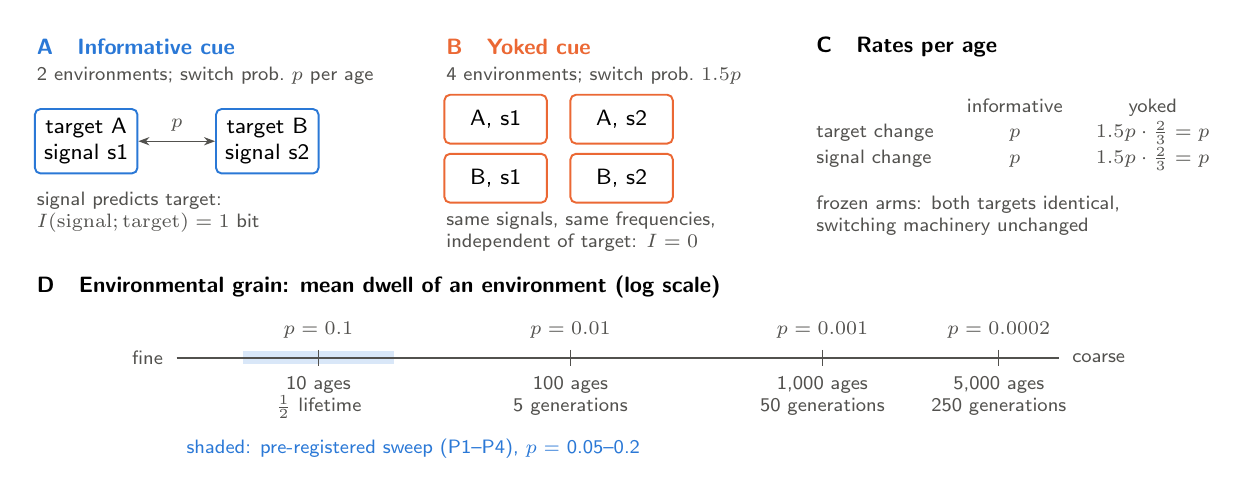
\begin{tikzpicture}[
  font=\sffamily\footnotesize,
  env/.style={draw=inktwo, rounded corners=2pt, minimum width=1.3cm, minimum height=0.62cm, align=center, fill=white},
  hdr/.style={font=\sffamily\footnotesize\bfseries, anchor=west},
  sub/.style={font=\sffamily\scriptsize, text=inktwo, anchor=west},
  lbl/.style={font=\sffamily\scriptsize, text=inktwo},
]
% --- A: informative
\node[hdr, text=cueinfo] at (0,3.25) {A\quad Informative cue};
\node[sub] at (0,2.88) {2 environments; switch prob.\ $p$ per age};
\node[env, draw=cueinfo, line width=0.7pt] (a1) at (0.75,2.05) {target A\\signal s1};
\node[env, draw=cueinfo, line width=0.7pt] (a2) at (3.05,2.05) {target B\\signal s2};
\draw[{Stealth[length=4pt]}-{Stealth[length=4pt]}, inktwo] (a1) -- node[above, lbl] {$p$} (a2);
\node[sub, align=left] at (0,1.15) {signal predicts target:\\$I(\mathrm{signal};\mathrm{target}) = 1$ bit};
% --- B: yoked
\node[hdr, text=cueyoked] at (5.2,3.25) {B\quad Yoked cue};
\node[sub] at (5.2,2.88) {4 environments; switch prob.\ $1.5p$};
\node[env, draw=cueyoked, line width=0.7pt] at (5.95,2.33) {A, s1};
\node[env, draw=cueyoked, line width=0.7pt] at (7.55,2.33) {A, s2};
\node[env, draw=cueyoked, line width=0.7pt] at (5.95,1.58) {B, s1};
\node[env, draw=cueyoked, line width=0.7pt] at (7.55,1.58) {B, s2};
\node[sub, align=left] at (5.2,0.9) {same signals, same frequencies,\\independent of target: $I = 0$};
% --- C: rate matching
\node[hdr] at (9.9,3.25) {C\quad Rates per age};
\node[sub, align=left] at (9.9,2.15) {
\begin{tabular}{@{}lcc@{}}
 & informative & yoked\\[1pt]
target change & $p$ & $1.5p\cdot\tfrac{2}{3} = p$\\[1pt]
signal change & $p$ & $1.5p\cdot\tfrac{2}{3} = p$\\
\end{tabular}};
\node[sub, align=left] at (9.9,1.1) {frozen arms: both targets identical,\\switching machinery unchanged};
% --- D: grain axis, logarithmic in mean dwell (x = 0.5 + 3.2 log10 dwell)
\node[hdr] at (0,0.2) {D\quad Environmental grain: mean dwell of an environment (log scale)};
\fill[cueinfo, opacity=0.18] (2.74,-0.78) rectangle (4.66,-0.62);
\draw[inktwo, line width=0.6pt] (1.9,-0.7) -- (13.1,-0.7);
\node[lbl, anchor=east] at (1.85,-0.7) {fine};
\node[lbl, anchor=west] at (13.15,-0.7) {coarse};
\foreach \x/\p/\d/\g in {3.70/0.1/10 ages/{$\tfrac12$ lifetime},6.90/0.01/100 ages/{5 generations},10.10/0.001/1{,}000 ages/{50 generations},12.34/0.0002/5{,}000 ages/{250 generations}} {
  \draw[inktwo] (\x,-0.6) -- (\x,-0.8);
  \node[lbl, above] at (\x,-0.58) {$p=\p$};
  \node[lbl, below, align=center] at (\x,-0.82) {\d\\\g};
}
\node[font=\sffamily\scriptsize, text=cueinfo, anchor=west] at (1.9,-1.85) {shaded: pre-registered sweep (P1--P4), $p$ = 0.05--0.2};
\end{tikzpicture}
\fi
\caption{{\bf Design.}
(A) Informative arm in R-Aevol: two environments, each target paired with its
own signal protein; the signal predicts the target.
(B) Yoked arm: four environments pairing each target with each signal, so the
same signals occur at the same frequencies but carry no information about the
target.
(C) Because a switch moves to a different environment chosen at random, the
yoked arm switches with probability $1.5p$, which equalises both the per-age
target-change and signal-change rates with the informative arm. Frozen arms
use two identical targets.
(D) Environmental grain as the mean dwell time of an environment, set by the
switching probability $p$ over the 20 ages of a lifetime. Ticks mark the four
switching probabilities of the grain experiment (G1--G4); shading marks the
range of the pre-registered sweep (P1--P4).}
\label{fig1}
\end{figure}

\subsection*{In EvoSim, fluctuation adds connections but not wiring strength}

We first measured connectivity in EvoSim, where earlier work had shown that
fluctuation raises connection density (S4~Text). In 180 populations (six arms
$\times$ 30 seeds, 150{,}000 time steps), fluctuation without a cue raised count
density---the fraction of possible connections that are non-zero---from 0.467 to
0.587 ($+25.5\%$, $p<10^{-4}$, $d=2.2$; survivors only, $n=28$ versus 30;
Fig~\ref{fig2}A). Over the same networks, strength density---summed absolute
connection weight divided by the number of possible connections---fell from 0.207
to 0.184 ($-10.9\%$, $p<10^{-4}$, $d=-1.4$; Fig~\ref{fig2}B). Total wiring
strength did not change (38.0 versus 37.5, $p=0.86$; Fig~\ref{fig2}C).
Fluctuation added connections without adding strength: the mean strength of a
non-zero connection fell by about 30\%. The same pattern held with an
informative cue and with a yoked one. Node count was near the minimum of 13 in
this regime and rose only slightly ($+0.6$ nodes, $p=0.047$).

Two features of this regime need stating. First, fluctuating populations were
40\% smaller than frozen ones, and population size can affect genome
architecture on its own. The population ranges of the two arms did not overlap,
so the two cannot be separated statistically; but within every arm, larger
populations had \emph{lower} strength density ($r=-0.39$; Fig~\ref{fig2}D), so
population size, taken at face value, predicts higher strength density in the
smaller fluctuating populations---the opposite of what we observed. Second, in
this regime the cue went unused: informative and yoked arms had identical
strength density ($p=0.99$). EvoSim organisms read the cue only when development
is made reversible, and even then exploit little of its information (S4~Text), so
EvoSim speaks mainly to fluctuation that cannot be tracked.

\begin{figure}[!ht]
\centering
\ifshowfigs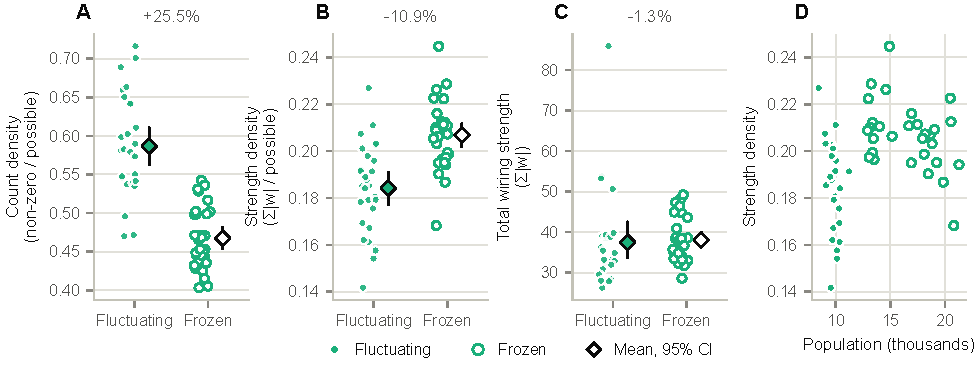
\includegraphics[width=\linewidth]{figures/fig2_evosim.pdf}\fi
\caption{{\bf EvoSim: more connections, less strength.}
Fluctuating (no cue; filled) versus frozen (hollow) populations, one point per
population; diamonds are means with bootstrap 95\% confidence intervals. Numbers
above panels are the change in the mean.
(A) Count density: non-zero connections divided by possible connections.
(B) Strength density: summed absolute weight divided by possible connections.
(C) Total wiring strength.
(D) Strength density against population size within each arm. Extinct
populations (2 of 30 fluctuating, 0 of 30 frozen) are excluded.}
\label{fig2}
\end{figure}

\subsection*{In R-Aevol, whether fluctuation strengthens regulation depends on a usable cue}

We next asked whether an independent model reproduced EvoSim's earlier
conclusions---that fluctuation raises genome size and connectivity, and that the
information content of a cue is irrelevant. It did not. In an exploratory
experiment (six arms $\times$ 12 seeds, 30{,}000 generations), fluctuation
\emph{reduced} genome size in every cue condition, and whether it strengthened
regulation depended on the cue (Fig~\ref{fig3}). With an informative cue,
fluctuating populations evolved total regulatory strength of 12.7 against 4.7 in
the frozen arm with the same signals; with no cue, fluctuating populations had
the weakest regulation of all six arms (1.4).

\begin{figure}[!ht]
\centering
\ifshowfigs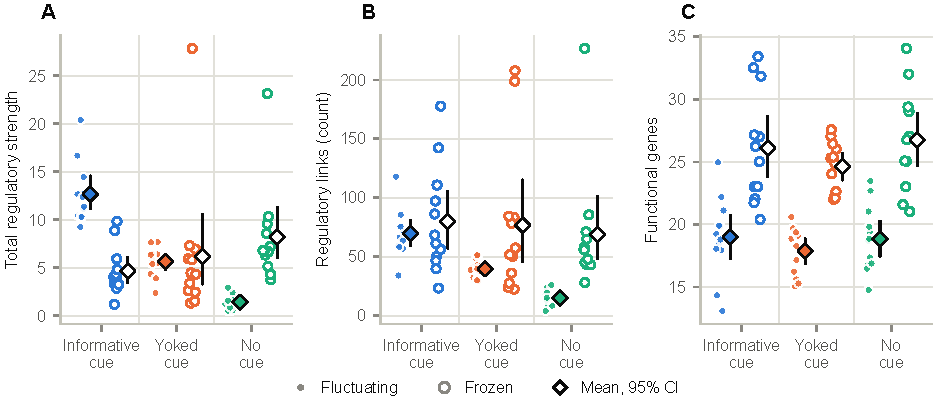
\includegraphics[width=\linewidth]{figures/fig3_raevol_v1.pdf}\fi
\caption{{\bf R-Aevol, six arms (exploratory).}
Total regulatory strength (A), number of regulatory links (B) and number of
functional genes (C) for each combination of environment (filled, fluctuating;
hollow, frozen) and cue (colour), one point per population; means with bootstrap
95\% confidence intervals. Switching probability 0.10, population 1024, 12
populations per arm.}
\label{fig3}
\end{figure}

Because this interpretation was formed after seeing the data, we tested it with
new seeds. Before running anything, we committed four predictions, their
measures, statistical tests and decision rules to version control
(Table~\ref{table2}; Materials and methods). The test varied the switching
probability over a fourfold range (0.05, 0.10 and 0.20 per age) at a population
of 1024, with 12 new seeds per cell, and repeated the central contrasts at a
population of 512. For the two predictions that depend on cue use we also
specified a manipulation check: that the informative cue lowers metabolic error
relative to the yoked one, i.e.\ that organisms actually use it. The check held at
switching probabilities 0.10 and 0.20 ($p<10^{-4}$) but not at 0.05
($p=0.088$), so by the pre-registered rule those predictions were judged at the
two faster rates only.

All four predictions were supported (Table~\ref{table2}, Fig~\ref{fig4}). With an
informative cue, fluctuation increased total regulatory strength over the frozen
environment 1.8-fold at $p=0.10$ and 2.7-fold at $p=0.20$ (P1; Holm-adjusted
$p=0.005$ and $\approx 10^{-4}$). Without a cue, fluctuation reduced it roughly
fivefold at every rate (1.1--1.2 against 6.3; P3; Holm-adjusted $p\approx10^{-4}$
at each rate). The slowest-switching informative cells, excluded from the
verdict, pointed the same way (11.0 against 5.9). One of these populations lost
every regulatory connection for the whole analysis window, the only such case in
the experiment.

\begin{figure}[!ht]
\centering
\ifshowfigs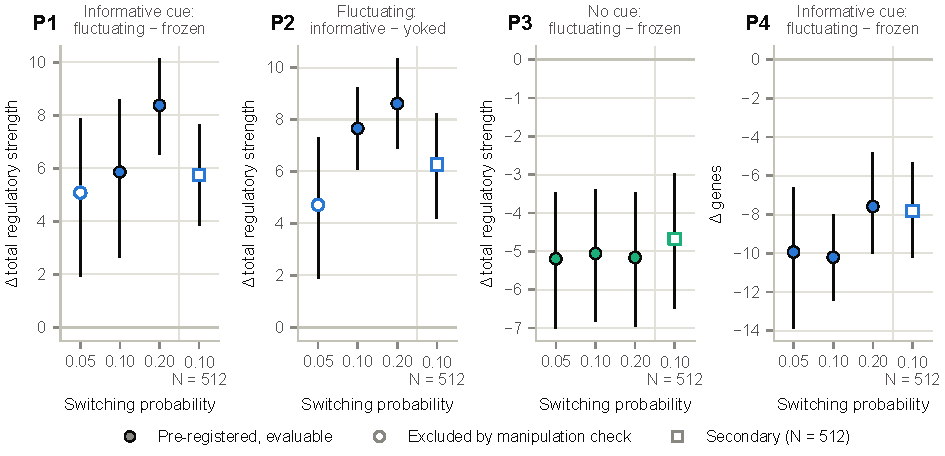
\includegraphics[width=\linewidth]{figures/fig4_preregistered.pdf}\fi
\caption{{\bf Pre-registered test.}
Differences in means with bootstrap 95\% confidence intervals for each
pre-registered contrast, at each switching probability (population 1024) and at
population 512 (squares; secondary, no verdict). Open circles: cells excluded
from the verdict because the manipulation check failed at that rate. For P3 at
population 512 the frozen baseline is the population-1024 frozen arm, the only
one run. P1: effect of fluctuation on total regulatory strength with an
informative cue. P2: informative minus yoked cue under fluctuation. P3: effect of
fluctuation without a cue. P4: effect of fluctuation on the number of functional
genes.}
\label{fig4}
\end{figure}

\subsection*{The cue's information, not its presence, is what matters}

The yoked control isolates information from stimulation: the informative and
yoked arms receive the same two signal proteins, at the same concentration and
frequency, switching at the same rate; only the contingency between signal and
target differs. Informative-cue populations evolved 2.3-fold ($p=0.10$) and
2.9-fold ($p=0.20$) greater regulatory strength than yoked ones (P2;
Holm-adjusted $p\approx10^{-4}$ at both) and matched the target roughly twice as
well (metabolic error 0.029 versus 0.058 at $p=0.10$); in the exploratory
experiment they also carried more transcription factors (11.2 versus 6.2). In a
frozen environment, where the signal still switches but announces nothing
because the target never changes, informative and yoked cues were
indistinguishable (7.5 versus 5.4, $p=0.18$). The difference between cue arms
therefore arises only when the cue carries information about something that
changes---the property the yoked design is built to isolate.

This reverses EvoSim's earlier conclusion that information content is
irrelevant. The two results are compatible once cue use is taken into account:
in the EvoSim regime where that conclusion was drawn, organisms exploited only
about a tenth of the information available to them (S4~Text), whereas R-Aevol
organisms halved their error when given an informative cue.

\subsection*{Fine-grained fluctuation shrinks the genome}

Fluctuation reduced the number of functional genes at every switching rate, by
10, 10 and 8 genes (26.3, 28.3 and 25.6 in frozen against 16.3, 18.1 and 18.0 in
fluctuating populations; P4; Holm-adjusted $p\le 3\times10^{-4}$;
Fig~\ref{fig4}), and at a population of 512 (25.3 against 17.5, $p<10^{-4}$). This
is the opposite of the genome enlargement reported for fluctuating selection in
other models~\cite{tsuda2010,bentkowski2015} and of EvoSim's own earlier finding
(S4~Text). One plausible mechanism is that in Aevol precision is bought with
genes: the phenotype is a sum of contributions from individual genes, so a
constant target that can be matched closely rewards additional genes, whereas a
target that switches within a lifetime cannot be matched closely and leaves a
coarser, cheaper phenotype. Frozen populations reached metabolic errors near
0.008, fluctuating ones without a usable cue near 0.06. We did not test this
mechanism.

\subsection*{Counting connections can give the wrong sign}

Connection counts and connection strength did not always move together
(Fig~\ref{fig5}). In EvoSim, fluctuation raised the count and lowered strength per
possible connection. In R-Aevol, informative-cue populations in a fluctuating
environment had \emph{fewer} raw regulatory links than their frozen counterparts
at every switching rate (0.60, 0.78 and 0.83 times as many), while their total
regulatory strength was 1.8--2.7 times higher and their strength per link
roughly twice as high. A connectivity measure based on counting links would
have concluded that fluctuation with a usable cue \emph{simplifies} regulatory
networks. Without a cue, by contrast, count and strength fell together (both to
about a fifth of the frozen value), so the two measures do not always disagree;
the point is that a count cannot be trusted to report strength. These
comparisons were specified in advance as secondary analyses and carry no verdict.

\begin{figure}[!ht]
\centering
\ifshowfigs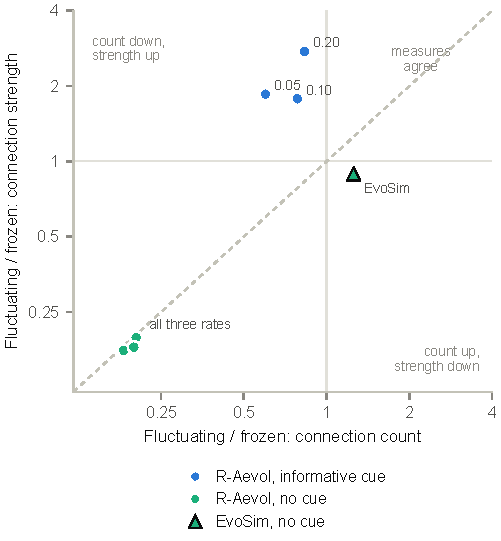
\includegraphics[width=0.62\linewidth]{figures/fig5_count_vs_strength.pdf}\fi
\caption{{\bf Counting versus weighing.}
Ratio of fluctuating to frozen connection count against the corresponding ratio
of connection strength, on logarithmic axes. R-Aevol (circles): raw number of
regulatory links and total regulatory strength, per switching probability,
population 1024. EvoSim (triangle): count density and strength density, no cue.
Points on the dashed diagonal are cases in which the two measures agree; points
off it are cases in which counting misreports strength, and points in the
upper-left or lower-right quadrants are cases in which it reports the wrong
sign.}
\label{fig5}
\end{figure}

\subsection*{Environmental grain}

To address the conflict with Tsuda and Kawata~\cite{tsuda2010}, who found that
cue-free fluctuation across generations promotes regulatory complexity, we
varied grain in R-Aevol without changing the model. The environment is a single
Markov chain over ages that continues from one generation to the next, so the
switching probability sets the mean time an environment persists: from half a
lifetime at $p=0.1$ to about 250 generations at $p=0.0002$ (Fig~\ref{fig1}D). We
predicted that coarse-grained cue-free fluctuation would produce larger genomes
and stronger regulation than fine-grained fluctuation (G1, G3) and than a frozen
environment (G2, G4)---Tsuda and Kawata's direction---and fixed in advance how
each outcome would be interpreted (Materials and methods).
\pending{results of the 60-run grain experiment, expected 2026-09-28}

\begin{figure}[!ht]
\centering
\ifshowfigs
\fcolorbox{pend}{white}{\parbox[c][1.3in][c]{0.8\linewidth}{\centering\sffamily\color{pend}
Fig 6 will show gene number and total regulatory strength against mean
environmental dwell time\\ for cue-free fluctuating populations, with the frozen mean for reference.\\[4pt]
\textbf{Results pending (grain experiment running).}}}
\fi
\caption{{\bf Environmental grain.} \pending{figure and legend}}
\label{fig6}
\end{figure}

% =============================================================================
\section*{Discussion}

Environmental fluctuation did not select for regulatory complexity as such. In
R-Aevol, whether it strengthened regulation depended on whether the organism
could tell which environment it was in: with an informative cue, fluctuation
produced the strongest regulation we observed; with none, the weakest. A yoked
cue that delivered the same molecules at the same rate did not substitute for an
informative one, so it was the information, not the stimulation, that mattered.
These conclusions held across switching rates and population sizes, in a test
whose predictions and analysis were fixed before the data existed.

This extends a well-established result at the level of the phenotype to the
level of architecture. That reliable cues favour plastic responses and their
absence favours generalism or bet-hedging is
classical~\cite{levins1968,moran1992,kussell2005,botero2015}, and has recently
been shown for the evolution of plasticity in a gene regulatory
network~\cite{jorritsma2026}. Our contribution is to show the corresponding
consequence for the network that implements the response---its regulatory
strength and its size---and to separate a cue's information from its presence,
which manipulations of cue reliability alone cannot do.

\pending{paragraph on grain and Tsuda \& Kawata. EvoSim's fluctuation is coarse
relative to a lifetime---development occurs once at birth and each environmental
state lasts on the order of twenty generations---and EvoSim earlier found genome
enlargement under fluctuation, as Tsuda and Kawata do; R-Aevol's fluctuation is
fine-grained and shrinks the genome. The grain experiment tests whether this is
the reconciling variable within one model.}

Counting connections and weighing them diverged in EvoSim and in R-Aevol's
informative-cue populations, for different reasons. In EvoSim, duplication and
node addition copy a node's connections with small added noise, so each copy
creates many weak connections where there were none; these persist when
purifying selection is weak, as it is in the smaller populations of a fluctuating
environment, and connection number rises while strength does not. In R-Aevol,
frozen populations carried more but weaker regulatory links, while
informative-cue populations carried fewer links of roughly twice the strength;
why frozen populations accumulate weak links we did not establish. In both cases
the count tracked something other than the function of the network. Since
connection counts are the usual measure of regulatory complexity in evolutionary
models~\cite{tsuda2010,espinosasoto2018,kashtan2005}, we suggest that claims about
connectivity report a weighted measure alongside or instead.

\subsection*{Limitations}
\begin{itemize}
\item \emph{One model for the trackable case.} The positive result---that a usable
cue lets fluctuation strengthen regulation---comes from R-Aevol. EvoSim organisms
read a cue only when development is reversible and exploit little of it; we have
not measured regulatory strength in that regime.
\item \emph{Replication depth.} Each R-Aevol cell has 12 populations, fewer than
the 60--100 common in comparable work~\cite{tsuda2010,lalejini2021}. The effects
are large (most $d>2$) and survive correction for multiple testing, but modest
effects would be missed.
\item \emph{Measures.} R-Aevol statistics describe the best individual in each
population at each generation, as the platform records them.
\item \emph{Environments.} R-Aevol's fluctuation alternates between two fixed
targets. It does not include the random walk to novel optima that Tsuda and
Kawata found most favourable to complexity~\cite{tsuda2010}.
\item \emph{Population size.} In EvoSim, fluctuation and population size are
confounded across arms; the within-arm evidence argues against population as
the explanation of the strength decline but cannot exclude it.
\item \emph{Genome size.} P4 confirms the direction of the genome-size effect, not
its mechanism.
\item \emph{A pre-registered confirmation that could not run.} We pre-registered a
confirmation of the EvoSim count--strength divergence in a regime with more
hidden nodes, conditional on fluctuating populations surviving there. They did
not (2 to 5 of 6 survived, against 6 of 6 frozen), so it was not run and the
EvoSim result remains exploratory.
\item \emph{Timestamps.} Pre-registrations were committed to version control
before the corresponding runs; for the first sweep these timestamps are local
and not independently verifiable.
\end{itemize}

\subsection*{Conclusion}
A changing world does not in itself build stronger regulation. It does so when
the organism has the information to track the change, and when it has not,
fluctuation leaves regulation weaker than a constant world would. Whether a model
reports otherwise may depend on whether it counts connections or weighs them.

% =============================================================================
\section*{Materials and methods}

\subsection*{EvoSim}
EvoSim is described in full, following the ODD protocol~\cite{grimm2020}, in
S1~Text; we summarise the parts relevant here. Organisms live on a $G\times G$
lattice ($G=128$) with six diffusing resource channels. Only the first receives
external inflow; consuming channel $r$ releases a byproduct into channel $r+1$,
with declining yields along the chain. Each organism carries an energy store,
divides when it exceeds a heritable threshold, and dies when energy runs out.

\paragraph*{Genome and development.} A genome is a weight matrix $W$ and bias
vector $b$ over $n_g$ nodes, $13 \le n_g \le 32$. Nodes 1--12 are read out as the
phenotype and node 13 receives the abiotic cue; hidden nodes $14,\dots,n_g$ carry
no fixed meaning. Development runs once, at birth: expression is initialised at
0.1 and updated eight times as
\begin{equation}
e_k \leftarrow \tanh\Big(b_k + \sum_m W_{mk}\, e_m + u_k\Big),
\end{equation}
where $u_k$ is the local concentration of resource $k$ for $k\le 6$, the cue for
$k=13$, and zero otherwise. Expression is then mapped to the twelve traits.

\paragraph*{Mutation.} At each birth, each weight receives an additive Gaussian
perturbation ($\sigma=0.25$) with probability $10^{-3}$, reduced by the organism's
heritable repair trait by up to 85\%. Structural mutations are gene silencing
(probability 0.002; zeroes a node's outgoing weights), gene duplication (0.002;
copies a node's regulatory role onto another with $\mathcal{N}(0,0.05^2)$ noise on
every copied weight), and addition or deletion of a hidden node (0.003 each; an
added node duplicates an existing one in the same way). Connection silencing
(probability 0.2 per birth) sets one randomly chosen weight to exactly zero;
without it, additive mutation makes density ratchet towards one. Each hidden node
costs 0.0015 and each non-zero weight $5\times10^{-5}$ energy units per time step.

\paragraph*{Environment and cue.} An abiotic condition cycles through discrete
states with a period of 2{,}000 time steps; each state rotates which resource
channel pays best, and 40\% of external inflow follows the favoured channel. The
condition is fed to node 13. Fluctuating arms use six states, frozen arms one.
The yoked cue replaces the condition's value with one generated on an
incommensurate period (a multiplier of $5+\varphi$), so that it cycles through the
same values without predicting the state; the no-cue arm sets the cue's gain to
zero. With a single state the cue is identically zero, so the three frozen arms
are identical runs and were analysed as one.

\paragraph*{Measures.} Count density is the number of weights with
$|w|>10^{-4}$ divided by $n_g^2$; strength density is $\sum|w|/n_g^2$ over all
$n_g^2$ weights, zeros included; total strength is $\sum|w|$. Each is computed per
organism at birth, averaged over the population at each logged time step, and
averaged over the final 20\% of the run. Populations that went extinct were
excluded and counted.

\paragraph*{Runs.} 180 runs: six arms $\times$ 30 seeds, 150{,}000 time steps each.
Runs are deterministic given the seed and bit-identical across thread counts.

\subsection*{R-Aevol}
We used the \texttt{aevol-7} branch of Aevol (commit \texttt{33277374},
\url{https://gitlab.inria.fr/aevol/aevol}) compiled with regulation enabled
(\texttt{-Dwith-raevol=ON}) and per-generation statistics enabled
(\texttt{-Dwithout-stats=OFF}); building on Apple Silicon required correcting a
hard-coded OpenMP library path (S2~Text). Parameters (Table~\ref{table1}) follow
the platform's own two-environment example (\texttt{examples/dynamic\_env}),
including its binding matrix, used unchanged in every run.

\paragraph*{Environments.} Each environment is a target function built from three
Gaussians. Target B is target A reflected about the midpoint of the phenotypic
axis; both have geometric area 0.152468. Fluctuating arms switch between A and B;
frozen arms use two copies of the same target (A for odd seeds, B for even) so
that the switching machinery runs identically but the organism experiences no
change. The environment is a Markov chain over ages that continues across
generations: at each of the 20 ages it moves, with probability $p$, to a different
environment chosen uniformly among the others. We confirmed in the source that
this is the switching the platform's SIMD engine performs (S2~Text).

\paragraph*{Signals and the yoked control.} Two signal proteins, taken unchanged
from the platform's \texttt{complex\_env} example, are present at concentration
0.9 during ages when their environment is active and absent otherwise.
Informative arm: two environments, (A, s1) and (B, s2). Yoked arm: four
environments, (A, s1), (A, s2), (B, s1), (B, s2). No-cue arm: no signals. In the
two-environment arm every switch changes both target and signal, so both change
at rate $p$ per age. In the four-environment arm a switch changes the target with
probability 2/3 and the signal with probability 2/3, so at switching probability
$1.5p$ both again change at rate $p$ per age.

\paragraph*{Measures.} R-Aevol records, each generation, statistics of the best
individual. Genome size is the number of functional genes. Total regulatory
strength $S = n_\mathrm{link}\times\bar{a}$, where $n_\mathrm{link}$ is the number of
protein--RNA influences and $\bar{a}$ their mean strength (the sum of enhancing and
operating factors divided by their number); $S=0$ when there are no links. Each
run is summarised by its mean over generations 25{,}001--30{,}000.

\paragraph*{Runs.} Exploratory: six arms $\times$ 12 seeds at $p=0.10$, population
1024 (72 runs). Pre-registered sweep: fluctuating informative, yoked and no-cue
arms and frozen informative arms at $p\in\{0.05, 0.10, 0.20\}$, frozen no-cue and
frozen yoked arms at $p=0.10$ (frozen no-cue is rate-independent), 12 new seeds
each, population 1024 (168 runs), plus the fluctuating informative, yoked and
no-cue arms and the frozen informative arm at population 512 (48 runs). Grain experiment:
cue-free fluctuating arms at $p\in\{0.1, 0.01, 0.001, 0.0002\}$ and a frozen arm, 12
new seeds each (60 runs). All completed runs reached 30{,}000 generations.

\begin{table}[!ht]
\centering
\caption{{\bf R-Aevol parameters.}}
\begin{tabular}{@{}ll@{}}
\toprule
Parameter & Value \\
\midrule
Population & 1024 ($32\times32$) or 512 ($32\times16$) \\
Selection & fitness-proportionate, pressure 750 \\
Point mutation, small insertion, small deletion & $5\times10^{-5}$ per base per generation \\
Duplication, deletion, translocation, inversion & $5\times10^{-5}$ per base per generation \\
Maximum indel size & 6 \\
Initial genome & 5{,}000 bases, one functional gene \\
Hill function & $n=4$, $\theta=0.5$ \\
Degradation & rate 1, 10 steps per age \\
Lifetime & 20 ages, fitness evaluated at all 20 \\
Binding matrix & fixed file from \texttt{examples/dynamic\_env}, all runs \\
Target sampling & 300 points \\
Signal concentration & 0.9 \\
Generations & 30{,}000 \\
\bottomrule
\end{tabular}
\label{table1}
\end{table}

\subsection*{Statistics}
The unit of analysis is a population. Each run contributes one number per
measure, so generations within a run are never treated as independent.
Differences between arms were tested with two-sided permutation tests on the
difference of means (100{,}000 permutations), with rank-based permutation tests
reported alongside. Multiple predictions were corrected with the Holm procedure.
Effect sizes are Cohen's $d$; intervals in figures are bootstrap 95\% confidence
intervals (10{,}000 resamples).

\subsection*{Pre-registration and deviations}
Predictions P1--P4, their measures, tests and decision rules, and the analysis
code were committed to version control (commit \texttt{f985ccd}) before the
pre-registered sweep was launched; the analysis was run once, on complete data,
with the committed code (verified by checksum). The only deviation was
operational: the host machine's idle sleep suspended runs overnight, which
lengthened wall time but cannot affect results, since runs are deterministic
given their seed. The EvoSim confirmation (commit \texttt{4bc16c3}) required
fluctuating and frozen populations to survive a viability pilot; none of the three
candidate regimes qualified and it was not run (commit \texttt{56fe3a0}). The
grain experiment was committed as \texttt{fa00777} \pending{OSF registration, if
made; outcome}.

\begin{table}[!ht]
\centering
\caption{{\bf Pre-registered predictions and verdicts.}}
\small
\begin{tabular}{@{}p{0.07\linewidth}p{0.6\linewidth}p{0.25\linewidth}@{}}
\toprule
Id & Prediction & Verdict \\
\midrule
P1 & Fluctuation with an informative cue raises total regulatory strength over frozen & supported ($p=0.10$, 0.20) \\
P2 & An informative cue raises it over a yoked cue & supported ($p=0.10$, 0.20) \\
P3 & Fluctuation without a cue lowers it below frozen & supported (all rates) \\
P4 & Fluctuation lowers the number of functional genes & supported (all rates) \\
P5 & EvoSim: count density up and strength density down in a regime above the node floor & not run (no viable regime) \\
G1--G4 & Coarse grain reverses the effect of cue-free fluctuation & \pending{running} \\
\bottomrule
\end{tabular}
\begin{flushleft}\footnotesize
Supported: the predicted sign at every evaluable rate and Holm-adjusted $p<0.05$
at two or more. Refuted: the opposite sign significant at any rate, or no rate
Holm-significant. Otherwise inconclusive. P1 and P2 are evaluable only at rates
where the informative cue measurably lowers metabolic error relative to the yoked
cue.
\end{flushleft}
\label{table2}
\end{table}

\subsection*{Software and availability}
EvoSim is written in Julia and depends only on the standard library for
simulation. R-Aevol runs were made on a single 12-core machine. All code---both
models' configurations, launchers, pre-registered analysis scripts and the full
history of the analyses---and the per-run statistics are available at
\pending{repository URL and Zenodo DOI}.

% =============================================================================
\section*{Supporting information}

\paragraph*{S1 Text.}
\label{S1_Text}
{\bf ODD description of EvoSim.} \pending{to be written}

\paragraph*{S2 Text.}
\label{S2_Text}
{\bf R-Aevol build, configuration files and the yoked-control derivation.}
\pending{to be written}

\paragraph*{S3 Table.}
\label{S3_Table}
{\bf Per-arm and per-run results for every experiment.} \pending{to be assembled}

\paragraph*{S4 Text.}
\label{S4_Text}
{\bf Earlier EvoSim results and the audit trail.} Claims that were superseded,
the measurement traps that produced them, and the control that caught each.
\pending{to be written}

\paragraph*{S5 Table.}
\label{S5_Table}
{\bf Prior-art comparison.} \pending{to be assembled}

\section*{Acknowledgments}
\pending{acknowledgements; disclosure of AI-assisted analysis and writing, as
required by PLOS policy}

\nolinenumbers
\bibliography{refs}

\end{document}
